\section{评估}
\label{sec:eval}

\begin{figure*}[t]
  \centering
  \setlength{\abovecaptionskip}{0pt}
  \setlength{\belowcaptionskip}{0pt}
  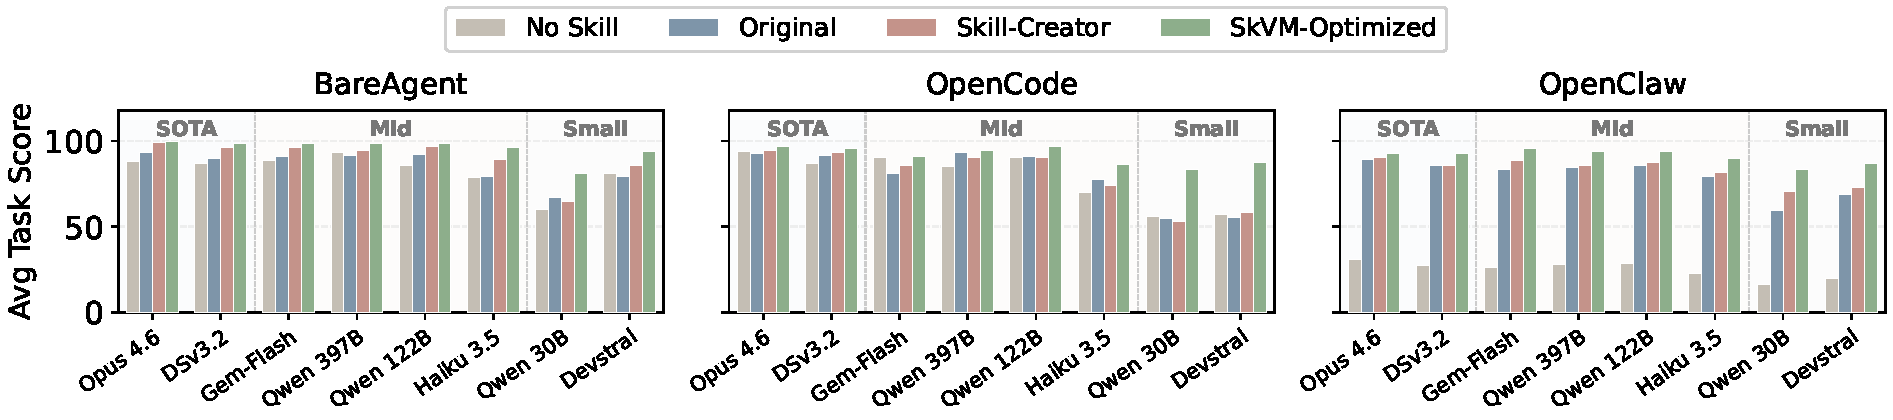
\includegraphics[width=\textwidth]{figures/e1_overview.pdf}
  \caption{各技能变体的平均任务分数。在八个模型与三个代理框架上比较四种变体：无技能、原始技能、Skill-Creator 和 \sys 优化技能。图中用底色区分 SOTA、中型与小型模型。\sys 优化技能始终取得最高分数，并且在较弱模型与 OpenClaw 上获得最大的绝对增益。}
  \label{fig:e1_overview}
\end{figure*}

\subsection{实验设置}
\label{sec:eval:setup}

\heading{基准。}
我们选择并扩展现有技能基准，包括 SkillsBench~\cite{li2026skillsbench} 和 PinchBench~\cite{pinchbench}，
覆盖代码生成、数据分析、文档创建和系统管理等多种代理任务。
每个任务至少配有一个来自主流技能来源的技能：Anthropic-skills~\cite{anthropic-skills-repo}、OpenClaw skills~\cite{openclaw} 和 skills.sh~\cite{skillssh}。
我们采用自动化评估套件，根据预定义标准进行静态分析与基于 LLM 的评估~\cite{zhu2024swebench, zheng2023llmasjudge}。

\heading{模型。}
我们在分属三个能力层级的八个模型上评估 \sys，以全面考察它在不同模型能力下的有效性。
\emph{SOTA}：claude-opus-4.6~\cite{claude4_6_opus}、deepseek-v3.2~\cite{deepseek2025v3}。
\emph{中型}：gemini-3-flash~\cite{gemini_flash}、qwen3.5-397b~\cite{qwen3_5_397b}、qwen3.5-122b~\cite{qwen3_5_122b}、claude-3.5-haiku~\cite{claude3_5_haiku}。
\emph{小型}：qwen3-30b~\cite{qwen3_30b}、devstral-small~\cite{devstral_small_2507}。

\heading{基线。}
我们将 \sys 与三个基线比较。
\emph{无技能}：代理在未加载任何技能的情况下执行。
\emph{原始技能}：使用原始技能。
\emph{Skill-Creator}：使用 Anthropic 的 Skill-Creator~\cite{anthropic-skill-creator} 配合 claude-opus-4.6 优化后的技能。

\heading{代理框架。}
我们选择三个不同的开源代理框架，以评估 \sys 在多样化执行环境中的性能。
各框架提供不同功能：
\emph{BareAgent} 是一个最小框架，不引入额外抽象层，直接把编译后的技能注入系统提示词。
\emph{OpenCode}~\cite{opencode} 是一个功能完整的代码代理框架，
支持批量工具分派，并提供丰富的代码执行工具集。
\emph{OpenClaw}~\cite{openclaw} 是一个通用代理框架，
集成了支持复杂多步任务执行的功能模块。

\heading{方法。}
我们首先对不同模型的原语能力进行画像，然后应用 \sys 的 AOT 与 JIT 编译，
为每个模型生成定制的优化技能变体。
为了支持编译后的技能产物，我们用自定义加载与管理机制扩展代理框架，使其能够执行 \sys 的优化。
对于每项任务，我们生成五个多样化输入实例，并测量平均任务完成率、token 消耗与端到端执行延迟。
所有实验均在配备 16GB 内存的 Mac Mini M4 上进行。

\begin{figure}[t]
  \setlength{\abovecaptionskip}{3pt}
  \setlength{\belowcaptionskip}{-5pt}
  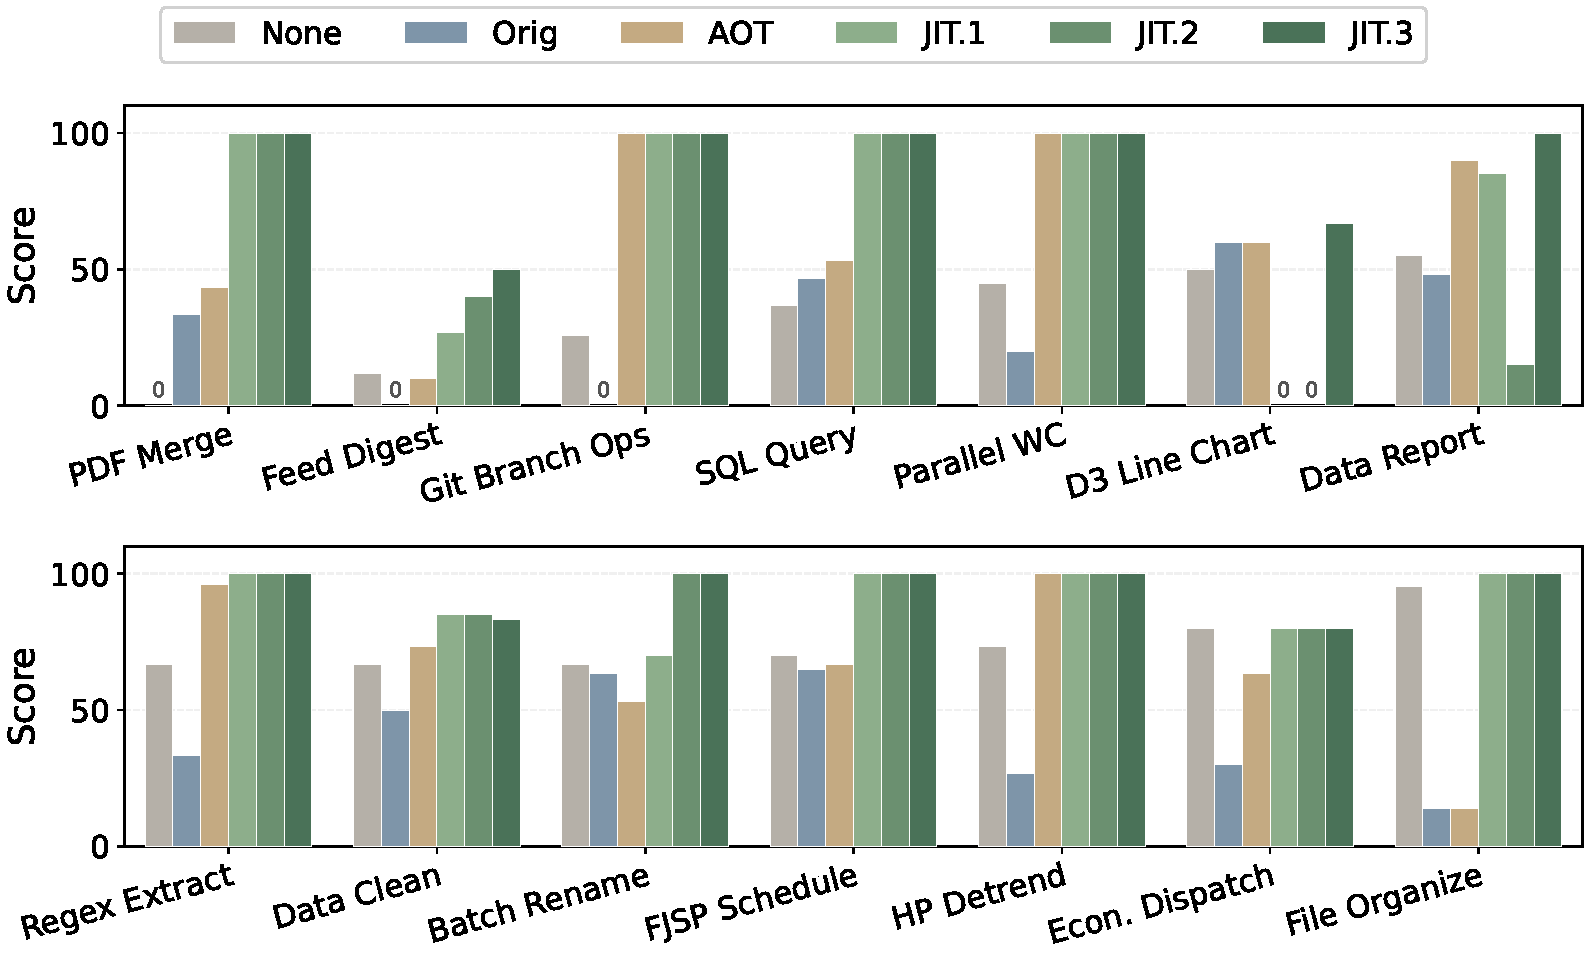
\includegraphics[width=\columnwidth]{figures/e6_skill_progression_bar.pdf}
  \caption{14 类技能上的分阶段优化拆解。每组展示六个阶段的分数：无技能、原始技能、AOT 编译技能，以及经过三轮 JIT 优化的技能。}
  \label{fig:e6}
\end{figure}

\subsection{技能编译的有效性}
\label{sec:eval:e1}

我们首先评估 \sys 提高任务完成率的有效性。
我们在不同任务、模型和代理框架上，将 \sys 优化的技能与未优化的基线技能比较。
对于 \sys，主要增益来自基于能力的编译与 JIT 优化。
图~\ref{fig:e1_heatmap} 展示了八个模型和三个代理框架上的编译效果。
单元格数值表示 \sys 优化后的任务完成率；单元格颜色表示相对于未优化基线技能的分数提升（绿色）或下降（红色）。

图~\ref{fig:e1_heatmap} 展示了 \sys 相对于原始技能，在多种模型与代理框架上的优化效果。
较弱模型从 \sys 优化中获益更多。
这一发现表明，对于大多数代理任务，较弱模型已经具备处理逻辑组成部分的足够能力，
但不擅长生成复杂 JSON 结构或管理环境依赖等非逻辑方面。
\sys 的编译优化通过细化原语能力来处理这些缺口，从而提高总体任务完成率。
对于较强模型，由于它们已经能够胜任任务，提升相对有限；
\sys 优化主要减少 token 消耗与执行延迟。
图~\ref{fig:e1_overview} 针对每个模型与代理框架，汇总了全部四种技能变体的平均任务分数。
在每一种模型--代理框架组合上，\sys 优化技能都取得最高分数。
随着模型能力降低，相对于 Skill-Creator 基线的提升会扩大：
在 BareAgent 上，\sys 优化技能相对于 Skill-Creator，在 qwen3-30b 上提升 25\%，在 devstral-small 上提升 10\%。
就性能下降而言，\sys 编译技能只在 4.5\% 的任务上降低任务完成率，而原始技能的对应比例为 15\%。
使用原始技能时，OpenCode 与 OpenClaw 之间的差异会随模型变化，最高达到 13 个百分点，
这表明仅代理框架行为本身就会实质性改变结果。
\sys 优化会同时提高两个框架上的分数，并将这种跨框架差距缩小至最多 5 个百分点。

\subsection{分阶段优化拆解}
\label{sec:eval:e6}

图~\ref{fig:e6} 分析了 Qwen3-30B 配合 BareAgent 时，
各优化阶段对 14 类技能的贡献。
每组展示六个阶段的分数：无技能、原始技能、AOT 编译技能，以及最多三轮 JIT 优化。
各轮所用任务类型相同，但内容不同。

在 14 类技能中，有 11 类使用原始技能时的表现不如无技能。
经过 \sys 的 AOT 编译，平均任务分数提高 88\%。
JIT 优化进一步识别 AOT 编译期间未暴露的能力缺陷，继续改善性能。
经过一轮 JIT 后，14 个技能中有 8 个在评估任务上取得满分；三轮后，有 10 个取得满分。

JIT 优化也可能造成性能下降。
例如，在折线图任务中，JIT 编译器向技能添加了示例文件，
但该文件过长并触发解析错误，致使分数下降。
经过由先前失败日志引导的三轮修订，JIT 编译器最终修复了该问题。

\subsection{编译带来的 Token 与成本效率}
\label{sec:eval:e2}

除了提高任务成功率，\sys 还通过减少 token 消耗，为 SOTA LLM 带来显著的成本收益。
LLM 可以在迭代式代理循环中根据环境反馈调整行动，从而纠正执行错误。
因此，即便任务最终成功，这一方法也可能浪费大量 token。
图~\ref{fig:e2_scatter} 展示了 \sys 编译后，不同模型层级与代理框架上的任务成功率和 token 成本如何变化。

评估显示，对于大多数模型与代理框架组合，\sys 编译会同时提高任务成功率并减少 token 消耗。
对于最强模型与最弱代理框架的组合（DS-v3.2 + BareAgent），我们观察到接近 40\% 的 token 节省。
产生这一提升的原因是：代理循环在纠正环境相关与工具调用错误时会产生交互开销，并且常常需要多次重试。
借助 JIT 编译，\sys 让模型完全避开这些错误路径，消除冗余交互并节省大量 token。

对于较弱模型，\sys 偶尔可能消耗更多 token。
这是因为 \sys 提高了任务完成率，使代理执行轨迹比使用基线技能时更长，
因而在边缘情形下会小幅增加 token 用量。

\begin{figure}[t]
  \centering
  \setlength{\abovecaptionskip}{5pt}
  \setlength{\belowcaptionskip}{-3pt}
  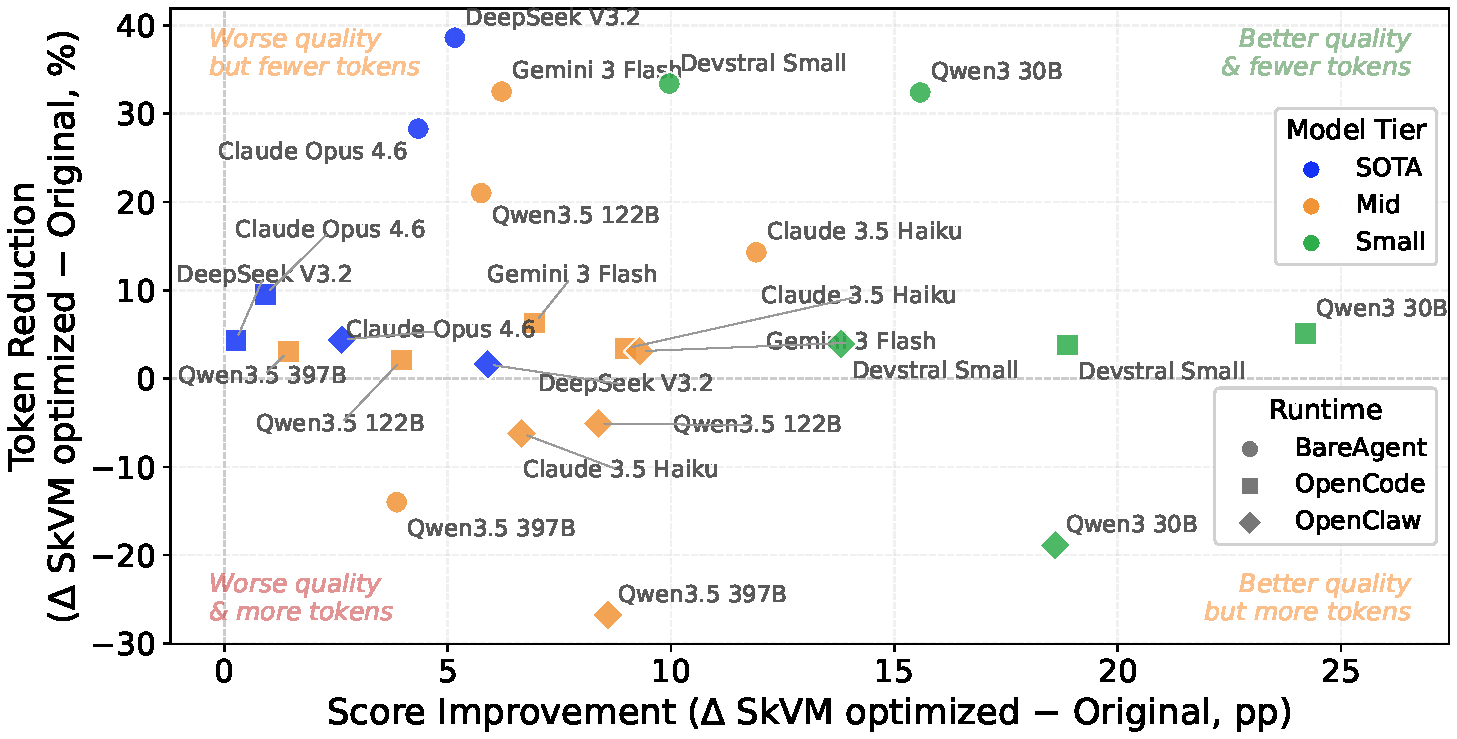
\includegraphics[width=\columnwidth]{figures/e2_scatter.pdf}
  \caption{相对于原始技能基线，\sys 优化带来的分数增益与 token 节省。每个点表示一个（模型，代理框架）组合；颜色表示模型层级，形状表示代理框架。大多数点位于右上象限：质量更高，token 也更少。}
  \label{fig:e2_scatter}
\end{figure}

\begin{figure}[t]
  \centering
  \setlength{\abovecaptionskip}{5pt}
  \setlength{\belowcaptionskip}{0pt}
  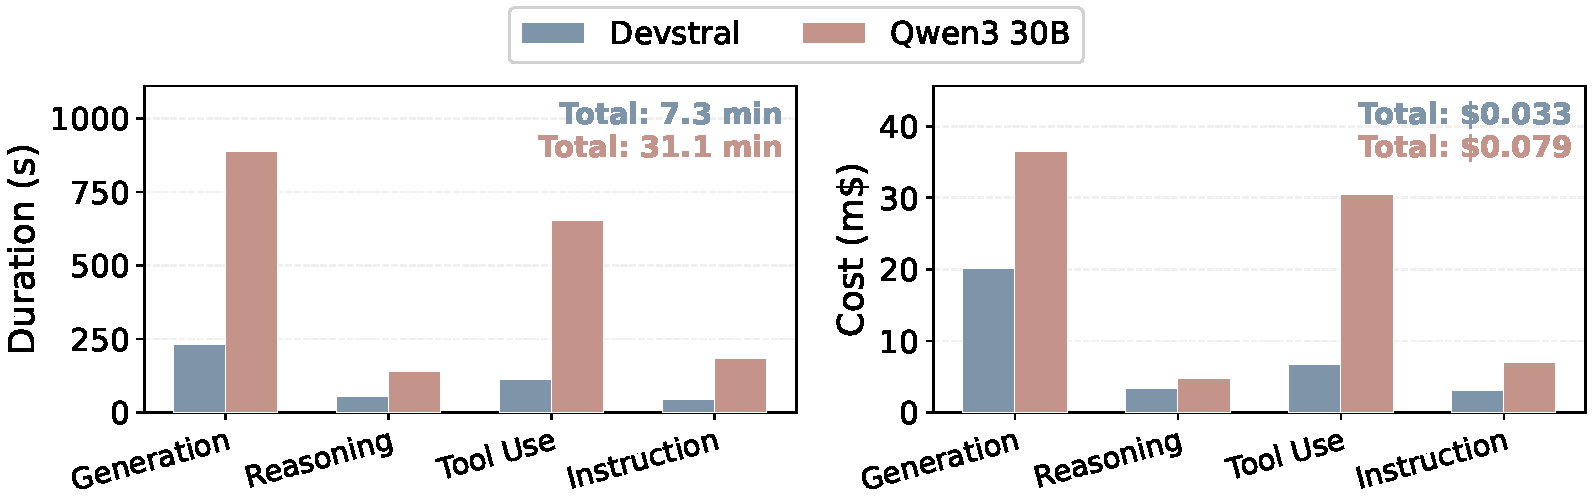
\includegraphics[width=\columnwidth]{figures/profiling_cost.pdf}
  \caption{两个小型模型的能力画像开销，按类别拆解。左：时长（秒）；右：成本（毫美元）。}
  \label{fig:profiling_cost}
\end{figure}

\begin{figure}[t]
\centering
\setlength{\abovecaptionskip}{3pt}
\setlength{\belowcaptionskip}{0pt}
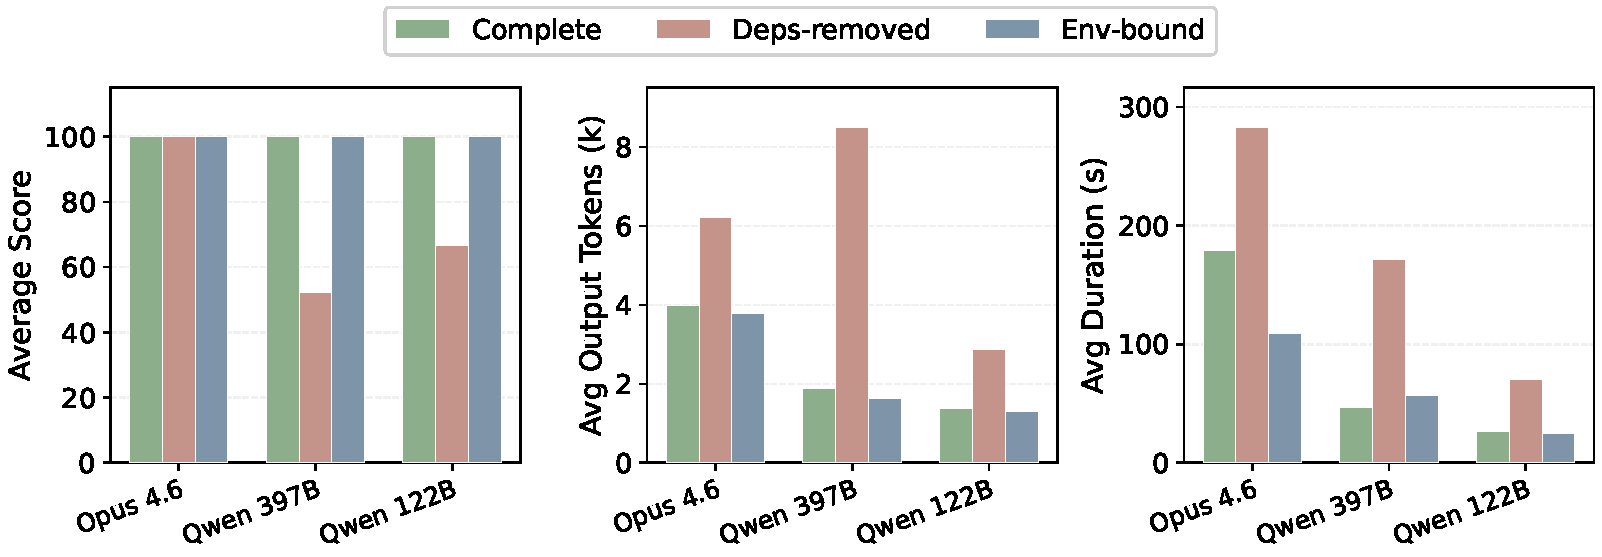
\includegraphics[width=\columnwidth]{figures/e3_env_adaptation.pdf}
\caption{环境绑定恢复了正确性、token 效率与执行速度。从左到右依次为：各模型在两个任务上的平均分数、平均 token 用量与平均时长。对三个模型而言，环境绑定后的性能都恢复到完整环境的水平。}
\label{fig:e3}
\end{figure}

\begin{figure*}[t]
  \centering
  \setlength{\abovecaptionskip}{3pt}
  \setlength{\belowcaptionskip}{0pt}
  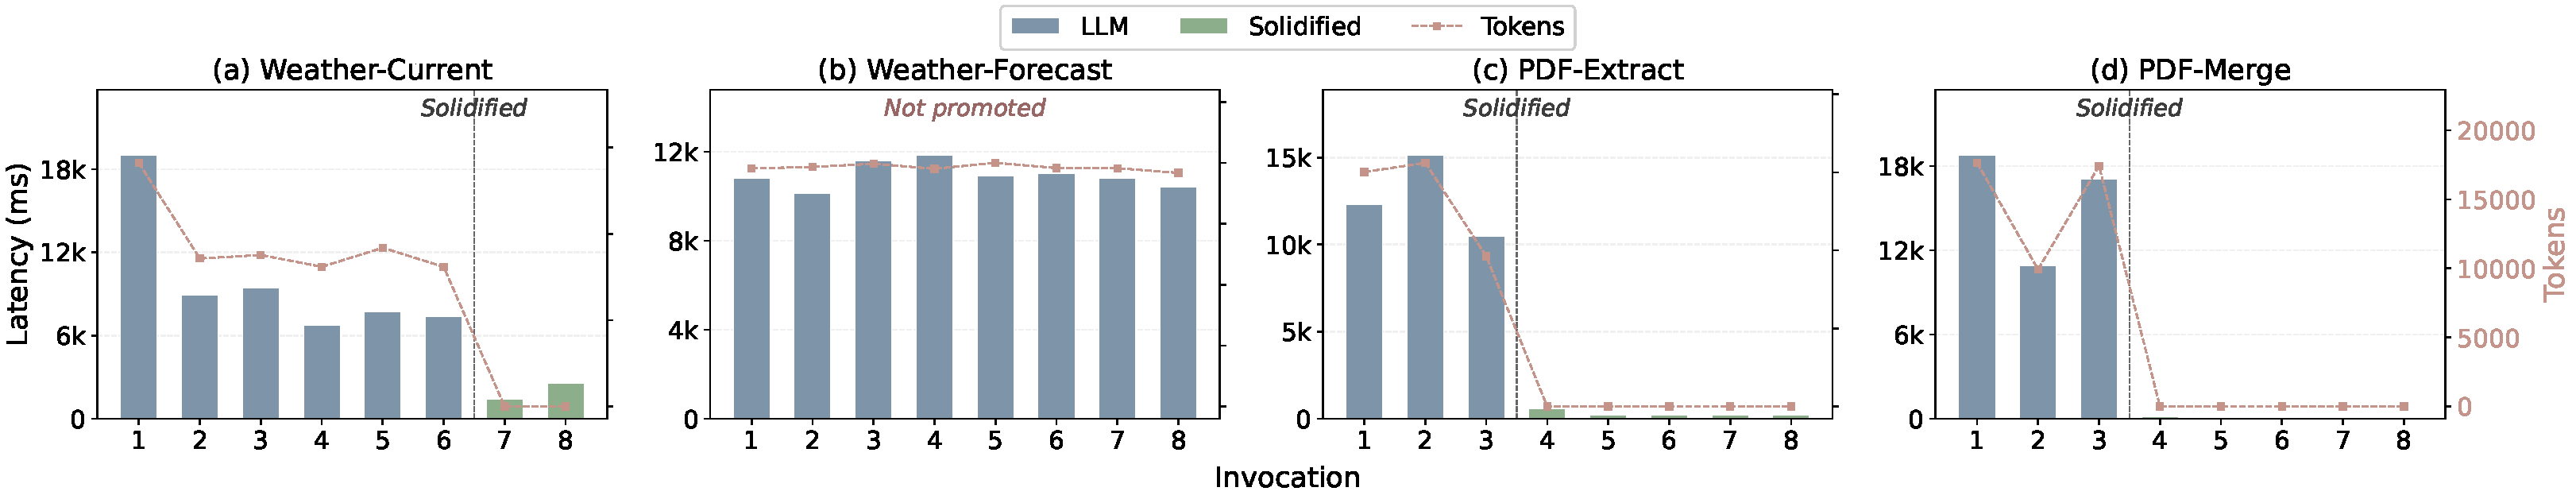
\includegraphics[width=\textwidth]{figures/e5_jit_demo.pdf}
  \caption{四个案例中的代码固化。蓝色柱表示 LLM 推理延迟，绿色柱表示固化后的执行延迟；虚线标出晋升点。Weather-forecast 从未晋升，因为运行时模型的代码模式偏离 AOT 预测，这验证了晋升门控作为安全机制的作用。}
  \label{fig:e5_jit}
\end{figure*}

\subsection{目标端画像的开销}
\label{sec:eval:profiling}

基于能力的编译要求对目标端进行一次画像，以构建其能力画像（\S\ref{sec:compiler:cap}）。
这种画像对于每个（模型，代理框架）组合只产生一次成本，
结果会被缓存，并复用于同一目标端后续的所有技能编译。
我们在两个小型模型 devstral-small 和 qwen3-30b 上测量了这一开销。

图~\ref{fig:profiling_cost} 展示了画像时长与成本按类别拆解的结果。
覆盖全部原语能力的完整画像，在 devstral-small 上用时 7.3 分钟，
在 qwen3-30b 上用时 31.1 分钟，成本分别为 \$0.033 和 \$0.079。

\subsection{环境绑定评估}
\label{sec:eval:e3}

前两个实验都在依赖完备的环境中进行测试。
然而在真实技能场景中，代理执行时缺少环境依赖十分常见。
解决这类环境问题对于较弱 LLM 构成显著挑战，并且经常导致技能执行失败。
\sys 在 AOT 编译阶段通过环境绑定机制处理这一问题。
该机制把环境依赖安装从 LLM 执行阶段前移到执行前的预处理阶段，使 LLM 只需专注于技能逻辑。

图~\ref{fig:e3} 展示了不同模型在三种环境配置下的性能：完整环境、采用环境绑定，以及缺少依赖。
claude-opus-4.6 等较强模型可以自行从依赖缺失中恢复，但代价是消耗更多 token。
对于 qwen3.5-122b 等较弱模型，依赖缺失会导致执行失败。
环境绑定能够完全恢复执行正确性，并大幅减少 token 消耗。

\subsection{并发性提取评估}
\label{sec:eval:e4}

\sys 从技能内部提取更多并行机会并提高效率。
我们评估三种并行类型：数据级并行（DLP）、指令级并行（ILP）和线程级并行（TLP）。
当单个技能内的指令批量处理大量独立数据时，可以应用 DLP。
当技能内有多条独立指令或代码段可并发执行时，可以应用 ILP。
当一个技能内运行多个独立子代理，且每个子代理处理无交叉依赖的自包含子任务时，可以应用 TLP。
图~\ref{fig:e4} 展示了 \sys 在这三种并行类型上的性能提升。

实验结果表明，\sys 的并行性提取策略实现最高 3.2$\times$ 的端到端加速。
TLP 的平均提升最大，因为其更粗粒度的并行性带来更显著的优化效果。
ILP 在指令层工作，能够同时减少执行时间与 LLM 调用次数。
DLP 的收益完全来自数据并行，因此性能提升会随数据并行度直接扩展。
我们还观察到，由于 LLM 吞吐波动以及代理循环迭代次数不同，
代理执行本身存在变化。因此，合理范围内的计时波动是可以接受的。

\begin{figure}[t]
\centering
\setlength{\abovecaptionskip}{5pt}
\setlength{\belowcaptionskip}{-5pt}
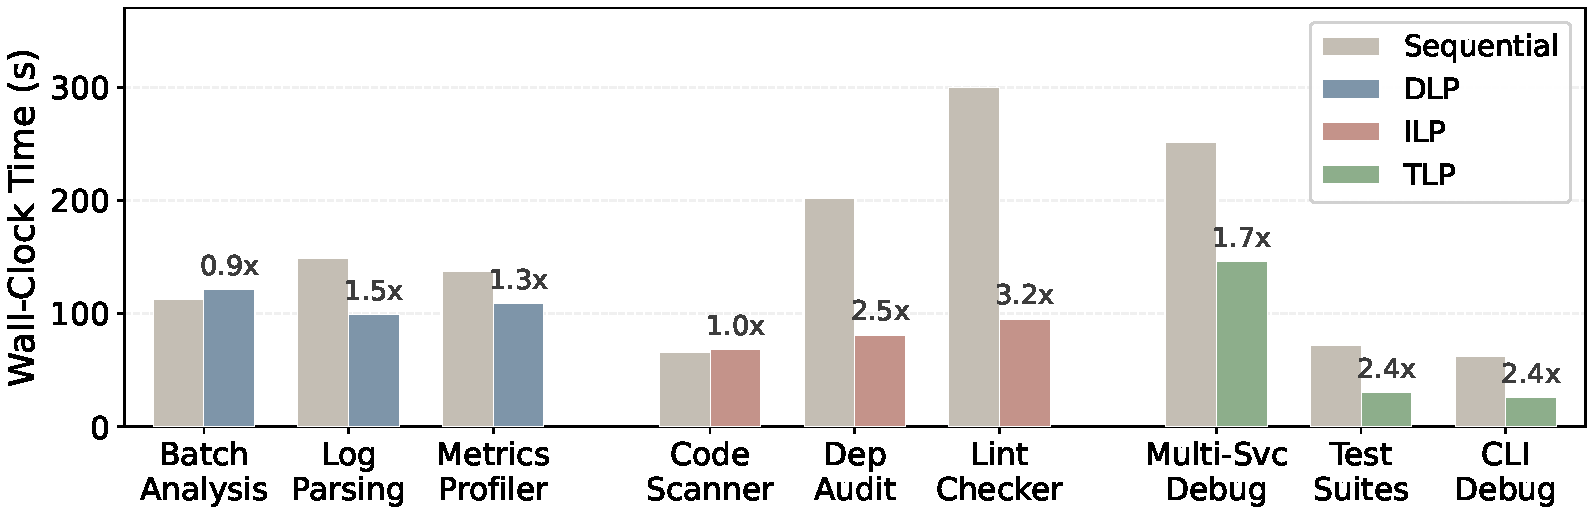
\includegraphics[width=\columnwidth]{figures/e4_parallelism.pdf}
\caption{八个任务上不同并行策略的性能。柱状图展示顺序执行、DLP、ILP 和 TLP。}
\label{fig:e4}
\end{figure}

\subsection{代码固化评估}
\label{sec:eval:e5}

我们进一步分析：采用 JIT 优化中的代码固化机制，
能否准确识别可复用代码段并提高代理执行效率。
如图~\ref{fig:e5_jit} 所示，我们对两个典型技能（天气、文档 PDF）进行详细分析。
对于两个 PDF 任务，尽管任务输入不同，LLM 生成的代码都与代码签名匹配。
因此，\sys 可以应用 JIT 编译优化，直接使用模板与输入参数生成固化代码。
对于 PDF-extract 任务，JIT 优化把执行时间从 10,469--15,116\,ms 降至 206--568\,ms，
实现 19--50$\times$ 加速。
在两个天气任务中，weather-current 需要调用外部天气 API，
其加速受网络延迟限制：执行时间从 9,000\,ms 降至 2,000\,ms，提升 5$\times$。
相比之下，weather-forecast 使用更灵活的格式，
因此生成的代码结构偏离代码签名，无法匹配。
于是，全部八次调用都依赖 LLM 生成，以避免调用错误代码。

如果固化代码执行导致任务失败，\sys 的安全机制会触发回退，
重新启用 LLM 代码生成以保证正确性。
